%\documentclass[draft]{beamer}
\documentclass{beamer}
%%%%%%%%%%%%%%%%%%%%%%%%%%%%%%%%%%%%%%%%%%%%%%%%%%%%%%%%%%%%%%%%%%%%%%%%%%%%
\let\Tiny=\tiny
\usefonttheme[onlymath]{serif}
\usepackage{bm}
\usepackage{amsmath}
\usepackage{amssymb}
\usepackage{microtype}
\usepackage{booktabs}
%%% INCLUDE FILE FOR DEFINITIONS
%%% These may require various packages.

% Shortcuts in regular text
\newcommand{\degs}{\ensuremath{^\circ}}
\newcommand{\EE}[1]{\ensuremath{\times 10^{#1}}}
\newcommand{\ttimes}{\ensuremath{{}\times{}}}
\newcommand{\cclicense}{%
  \smash{\raisebox{-0.45ex}{%
  \setlength{\unitlength}{1em}%
  \begin{picture}(1,1)%
    \put(0.5,0.5){\circle{1}}
    \put(0.5,0.5){\hbox to 0pt{\hss\raisebox{-.45ex}{\tiny\textsf{CC}}\hss}}
  \end{picture}%
  }}%
  \hskip -1em%
  \href{http://creativecommons.org/licenses/by-nc-sa/3.0/}%
  {\ \hskip 1em \textsf{BY-NC-SA}}%
}

%\newcommand{\horizsep}{{\par\noindent\centering\rule[.25ex]{.75\columnwidth}{2pt}\par}}
\newcommand{\horizsep}{\vspace{\baselineskip}\noindent\hspace{\stretch{1}}$
\ast\qquad \ast\qquad \ast\qquad
$ \hspace{\stretch{1}} \vspace{\baselineskip}}
\newcommand{\pytrt}{\textsf{PyTRT}}

% Research
\newcommand{\lop}[1]{\mathcal{L}\!\left[#1\right]}
\newcommand{\lopinv}[2]{\mathcal{I}_{#1}\!\left[#2\right]}
\newcommand{\Dtens}{\mat{D}}
\newcommand{\Etens}{\mat{E}}
\newcommand{\Identitytens}{\mat{I}}
\newcommand{\APone}{AP$_1$}
\newcommand{\Pone}{P$_1$}
\newcommand{\SN}{S$_N$}%{S$_\text{N}$}%{$S_N$}%
\newcommand{\PN}{P$_N$}%{P$_\text{N}$}%{$P_N$}%
\newcommand{\CN}{Crank--Nicolson} %Yes, it's Nic not Nich
\newcommand{\Eddington}{\mathcal{E}} %whatever symbol I decided for Eddington
\newcommand{\RadEn}{E} %whatever symbol I decide for radiation energy
\newcommand{\Sigmatr}{\Sigma_{\mathit{tr}}}

% Program names
\newcommand{\cpp}{\textsf{C\raisebox{0.2ex}{++}}}

% General math shortcuts
\newcommand{\ud}{\mathop{}\!\mathrm{d}}
\newcommand{\pder}[2]{\frac{\partial #1}{\partial #2}}
\newcommand{\oder}[2]{\frac{\mathrm{d} #1}{\mathrm{d} #2}}
\newcommand{\tpder}[2]{{\partial #1}/{\partial #2}} %inlined
\newcommand{\toder}[2]{{\mathrm{d} #1}/{\mathrm{d} #2}} %inlined
\newcommand{\lra}{ \quad \Longrightarrow \quad }
\newcommand{\eexp}{\mathop{}\!\mathrm{e}} % upright ``e'' for exponent
\newcommand{\expp}[1]{\exp\!\left( {#1} \right)} % exp with parentheses
\newcommand{\qeq}{\stackrel{\mathrm{?}}{=}}

% Probability
\newcommand{\expectation}[1]{\mathop{}\!\mathrm{E}\!\left[ #1 \right]}
\DeclareMathOperator{\Var}{Var} % variance

% Asymptotic analysis
\DeclareMathOperator{\Ei}{Ei} % Exponential function
\newcommand{\lapl}[1]{\mathcal{L}[{#1}]} %laplace

%change the Re and Im operators from fancy curly letters
\DeclareMathOperator{\MathOpRe}{Re}
\renewcommand{\Re}{\MathOpRe}
\DeclareMathOperator{\MathOpIm}{Im}
\renewcommand{\Im}{\MathOpIm}

%imaginary ``i'' , upright 'i' or \imath
\newcommand{\iimag}{\mathrm{i}}

% Finite differences
\newcommand{\hot}{\text{h.o.t.}}
\newcommand{\inv}{^{-1}}

% Numerical Linear Algebra
\newcommand{\conj}{^{\ast}} % complex conjugate (transpose)
\newcommand{\norm}[1]{\left\| #1 \right\|} % double pipe
\newcommand{\abs}[1]{\left| #1 \right|} % single pipe
\newcommand{\eps}{\varepsilon}
\DeclareMathOperator{\fl}{fl}

\DeclareMathOperator{\acosh}{arccosh} 

% Define a command to write a nice-looking element, e.g. 4,2 He
\newcommand{\elem}[3]{\ensuremath{{}^{{#1}}_{{#2}}\mathrm{{#3}}}}

% Vector definitions
\newcommand{\mat}[1]{\mathbf{#1}} %matrix is bold upright
\renewcommand{\vec}[1]{\bm{#1}} %vector is bold italic
\newcommand{\op}[1]{\mathsf{#1}} % ``operator'' is sans serif

\newcommand{\vd}{\bm{\cdot}} % slightly bold vector dot
\newcommand{\del}{\vec{\nabla}} % gradient (Del) is bold
\newcommand{\grad}{\vec{\nabla}} % gradient

%\newcommand{\abr}[1]{\langle {#1} \rangle}
\newcommand{\abr}[1]{\left\langle {#1} \right\rangle} % angle brackets for avg.

%% topbox is useful in extended definitions of math terms inside an align
\newcommand{\topbox}[2][0.6]{\parbox[t]{#1\columnwidth}{\raggedright{}#2}}

% commands to make text in math mode appear as zero-width (better-looking
% integrals/sums, e.g.)
% from mathmode.pdf page 74, or Alexander R. Perlis ``A complement to \smash,
% \llap, and \rlap''

\def\mathllap{\mathpalette\mathllapinternal}
	\def\mathllapinternal#1#2{%
	\llap{$\mathsurround=0pt#1{#2}$}%
}
\def\clap#1{\hbox to 0pt{\hss#1\hss}}%
\def\mathclap{\mathpalette\mathclapinternal}%
\def\mathclapinternal#1#2{%
	\clap{$\mathsurround=0pt#1{#2}$}%
}
\def\mathrlap{\mathpalette\mathrlapinternal}%
\def\mathrlapinternal#1#2{%
	\rlap{$\mathsurround=0pt#1{#2}$}%
}

\setSRJthesisfigurepaths

\definecolor{lightgray}{gray}{0.85}
%%%%%%%%%%%%%%%%%%%%%%%%%%%%%%%%%%%%%%%%%%%%%%%%%%%%%%%%%%%%%%%%%%%%%%%%%%%%

%30 minute presentation
%15 minutes scheduled for questions
%1 hour allotted total

\usetheme{AnnArbor}
\usecolortheme{seahorse}
\usecolortheme{orchid}
\setbeamercolor*{frametitle}{use=structure,bg=structure.fg!20!white}
\setbeamercolor*{frametitle right}{use=structure,bg=structure.fg!20!white}
\setbeamertemplate{navigation symbols}{\insertframenavigationsymbol}
\setbeamertemplate{caption}[numbered]

\title[Flatland Diffusion]%
{Diffusion Boundary Conditions in Flatland Geometry}

\author[SRJ, EWL]{Seth~R.~Johnson \and Edward~W.~Larsen}

\institute[UMich]{
University of Michigan, Ann Arbor
}
\date[11/1/2011]{November 1, 2011}

%\AtBeginSection[]
%{
%\begin{frame}
%  \frametitle{Outline}
%  \tableofcontents[currentsection]
%\end{frame}
%}

\hypersetup{colorlinks=true,linkcolor=black}

% only show section headings in table of contents
\setcounter{tocdepth}{1}

%use symbols for footnote
\renewcommand{\thefootnote}{\fnsymbol{footnote}}

\begin{document}
%%%%%%%%%%%%%%%%%%%%%%%%%%%%%%%%%%%%%%%%%%%%%%%%%%%%%%%%%%%%%%%%%%%%%%%%%%%%

\begin{frame}
\titlepage
\begin{center}
  
\includegraphics[width=0.2\textwidth]{umlogo}
\end{center}
\smash{
\includegraphics[width=0.2\textwidth]{neup-small}}
\end{frame}

%%%%%%%%%%%%%%%%%%%%%%%%%%%%%%%%%%%%%%%%%%%%%%%%%%%%%%%%%%%%%%%%%%%%%%%%%%%%
%\begin{frame}
%  \frametitle{Outline}
%  \tableofcontents
%\end{frame}
%%%%%%%%%%%%%%%%%%%%%%%%%%%%%%%%%%%%%%%%%%%%%%%%%%%%%%%%%%%%%%%%%%%%%%%%%%%%
\section{Introduction}
%%%%%%%%%%%%%%%%%%%%%%%%%%%%%%%%%%%%%%%%
\begin{frame}{What is flatland?}
  \begin{itemize}
    \item Fictional two-dimensional universe \cite{Abb1884} in which particles
      are constrained to exist and travel in a 2-D plane
    \item Multi-dimensional geometry with simpler direction variable
      \begin{itemize}
        \item Flatland: $(x,y,\omega)$; 2-D: $(x,y,\mu,\omega)$
        \item Polar cosine is set to zero
      \end{itemize}
    \item Useful testbed for methods development
      \begin{itemize}
        \item Smaller phase space means computationally cheaper
        \item Angle-dependent quantities are easier to visualize
      \end{itemize}
  \end{itemize}
\end{frame}

%%%%%%%%%%%%%%%%%%%%%%%%%%%%%%%%%%%%%%%%
\begin{frame}{Channel surfing}
\begin{center}
  How do you design a 2-D test problem to model axial behavior in
  a channel?
\end{center}
\vspace{-.75in}

\begin{minipage}[c]{2.25in}%
  \vspace{.75in}%
  \includegraphics<1-2>[width=2in]{chord-flatland}%
  \includegraphics<3>[width=2in]{channel-xy}%
\end{minipage}
\begin{minipage}[c]{2.25in}%
  \rule{0pt}{3in}%
  \includegraphics<2>[width=2in]{chord-xyz}%
  \includegraphics<3>[width=2in]{channel-xyz}%
\end{minipage}
\end{frame}

%%%%%%%%%%%%%%%%%%%%%%%%%%%%%%%%%%%%%%%%
\begin{frame}{Motivation}
  \begin{itemize}
    \item Testing new methods in flatland requires existing methods to be fully
      formulated in flatland
    \item Flatland diffusion has been derived \cite{Asa2008} but without
      boundary conditions
    \item Realistic systems are finite; computers are finite; boundaries are
      important
  \end{itemize}
\end{frame}

%%%%%%%%%%%%%%%%%%%%%%%%%%%%%%%%%%%%%%%%%%%%%%%%%%%%%%%%%%%%%%%%%%%%%%%%%%%%
\section{Theory}
\subsection{Transport}
\begin{frame}{Transport equation}

\begin{equation}\label{eq:generalTransport}
  \vec{\Omega}\vd \grad \psi + \sigma \psi
  = \frac{c \sigma}{\gamma_0} \int_{S} \psi \ud\Omega + \frac{q}{\gamma_0}
  \quad \vec{x}\in V,\ \vec{\Omega}\in S \,,
\end{equation}

  \vspace{2ex}

  \small
  \centering
  Angular variables:
  \begin{tabular}{rccc}
\toprule
   Geometry & $\vec{\Omega}=(\Omega_x, \Omega_y)$ & Domain $S$ & $\ud\Omega$
\\ \midrule
2-D & $( \sqrt{1-\mu^2} \cos \omega,
   \sqrt{1-\mu^2} \sin \omega)$
   & $-1 \le \mu \le 1$, $0 \le \omega < 2\pi$ & $\ud\mu \ud \omega$
   \\
   Flatland & $ ( \cos \omega, \sin \omega )$
   & $0 \le \omega < 2\pi$ & $\ud \omega$
\\ \bottomrule
  \end{tabular}

  \vspace{2ex}

Angular moments:
  \centering
  \begin{tabular}{rccc}
\toprule
   Geometry
   & $\gamma_0 \equiv \int_S \ud\Omega$
   & $\gamma_1 \equiv \int_S \abs{\vec{\Omega}\vd\vec{i}} \ud\Omega$
   & $\gamma_2 \equiv \int_S (\vec{\Omega}\vd\vec{i})^2 \ud\Omega$
\\ \midrule
   2-D & $4\pi$ & $2\pi$ & $\frac{4\pi}{3}$
   \\
   Flatland & $2\pi$ & $4$ & $\pi$
\\ \bottomrule
  \end{tabular}

\end{frame}

%%%%%%%%%%%%%%%%%%%%%%%%%%%%%%%%%%%%%%%%
%\begin{frame}{Monte Carlo sampling}
%Example of lower computational cost of flatland transport: isotropic volume
%source
%\begin{equation}\label{eq:volumeSourcePdf}
%  f(\vec{\Omega}) \ud\Omega = \frac{\ud\Omega}{\gamma_0} \,,
%  \quad \vec{\Omega} \in S\,.
%\end{equation}
%
%\begin{columns}
%  \column{.5\textwidth}
%  \begin{block}{2D}
%\begin{multline*}
%  f(\mu,\omega) \ud\mu\ud\omega = \frac{\ud\mu}{2}\frac{\ud\omega}{2\pi} \,,
%  \\
%  -1\le \mu \le 1,\ 0 \le \omega < 2\pi\,,
%\end{multline*}
%\begin{equation*}
%  \omega = 2\pi \xi_1\,, 
%  \mu = \sqrt{ \xi_2} \,, 
%\end{equation*}
%  \end{block}
%
%  \column{.5\textwidth}
%  \begin{block}{Flatland}
%\begin{equation*}
%  f(\omega) \ud\omega = \frac{\ud\omega}{2\pi} \,,
%  \quad 0 \le \omega < 2\pi\,,
%\end{equation*}
%\begin{equation*}
%  \omega = 2\pi \xi_1\,.
%\end{equation*}
%  \end{block}
%\end{columns}
%\end{frame}

%%%%%%%%%%%%%%%%%%%%%%%%%%%%%%%%%%%%%%%%
\subsection{Diffusion interior}
\begin{frame}{Linear-in-angle approximation}
The diffusion approximation begins by assuming that $\psi$ is linear in angle:
\begin{equation*}
  \psi(\vec{x}, \vec{\Omega}) \approx f(\vec{x}) + \vec{\Omega} \vd
  \vec{g}(\vec{x})\,.
\end{equation*}
The zeroth angular moment of $\psi$ determines $f$:
\begin{equation*}
  \phi = \int_S \psi \ud\Omega
= \int_S \left( f + \vec{\Omega}\vd \vec{g} \right) \ud\Omega
= \int_S\ud\Omega f + 0
= \gamma_0 f \,,
\end{equation*}
and the first moment of $\psi$ determines $g$:
\begin{equation*}
  \vec{J} = \int_S \vec{\Omega} \psi \ud\Omega
= f \int_S \vec{\Omega} \ud\Omega
  + \vec{g} \vd \int_S \vec{\Omega}\vec{\Omega} \ud\Omega
= \gamma_2 \vec{g} \,.
\end{equation*}
\only<1>{%
This is the \Pone\ approximation to the angular flux:
\begin{equation}\label{eq:ssPone}
  \psi(\vec{x}, \vec{\Omega})
  \approx \frac{1}{\gamma_0} \phi(\vec{x})
  + \frac{1}{\gamma_2} \vec{\Omega} \vd \vec{F}(\vec{x})\,.
\end{equation}%
}%
\only<2>{%
This is the \alert{2-D} \Pone\ approximation to the angular flux:
\begin{equation*}
  \psi(\vec{x}, \vec{\Omega})
  \approx \frac{1}{4\pi} \phi(\vec{x})
  + \frac{3}{4\pi} \vec{\Omega} \vd \vec{F}(\vec{x})\,.
\end{equation*}%
}%
\only<3>{%
This is the \alert{flatland} \Pone\ approximation to the angular flux:
\begin{equation*}
  \psi(\vec{x}, \vec{\Omega})
  \approx \frac{1}{2\pi} \phi(\vec{x})
  + \frac{1}{\pi} \vec{\Omega} \vd \vec{F}(\vec{x})\,.
\end{equation*}%
}%
\end{frame}

\begin{frame}{Fick's law}
The linear-in-angle approximation is a spherical harmonics closure to the
transport equation.

Operate on \eqref{eq:generalTransport} by $\int_S \vec{\Omega} (\cdot)
\ud\Omega$ and substitute \eqref{eq:ssPone}:
\begin{align*}
  \grad \vd \int_S \vec{\Omega} \vec{\Omega} \left(
  \frac{1}{\gamma_0}\phi + \frac{1}{\gamma_2} \vec{\Omega} \vd \vec{J}
  \right)
  \ud\Omega
  + \sigma \vec{J}
  &=
  \frac{c\sigma}{\gamma_0} \phi \int_S \vec{\Omega} \ud\Omega
  + \frac{1}{\gamma_0} q \int_S \vec{\Omega} \ud\Omega
  \\
  \frac{\gamma_2}{\gamma_0} \grad \phi + \sigma \vec{J} &= 0 \,.
\end{align*}

Solve for $\vec{J}$:
\begin{equation} \label{eq:fickGeneral}
  \vec{J}(\vec{x})
  = - \frac{\gamma_2}{\gamma_0} \frac{1}{\sigma(\vec{x})} \grad \phi(\vec{x})
  \equiv -D(\vec{x}) \grad \phi(\vec{x})\,.
\end{equation}

\begin{equation*}
  \text{2-D: } D = \frac{1}{3\sigma} \qquad
  \text{Flatland: } D = \frac{1}{2\sigma}\,.
\end{equation*}
\end{frame}

%%%%%%%%%%%%%%%%%%%%%%%%%%%%%%%%%%%%%%%%
\subsection{Diffusion Marshak boundary condition}
\begin{frame}{Marshak boundary condition}
  Heuristic: preserve the incident current (particle rate/flux) on the boundary

\begin{align*}
\int_{\vec{\Omega}\vd \vec{n} < 0 } \abs{\vec{\Omega}\vd \vec{n}}
\psi^b \ud\Omega
 &= 
\int_{\vec{\Omega}\vd \vec{n} < 0 } \abs{\vec{\Omega}\vd \vec{n}} 
 \frac{1}{\gamma_0} \left[ \phi - \frac{1}{\sigma}
  \vec{\Omega} \vd \grad \phi \right]
  \ud\Omega
\\
J^{-}
&=
\frac{1}{\gamma_0} \phi \left( \frac{\gamma_1}{2} \right) 
  + \frac{1}{\gamma_0}\frac{1}{\sigma} \left( \vec{n} \vd
  \frac{\gamma_2}{2} \Identitytens \right)
  \vd \grad \phi
\\
J^{-}
&=
\frac{\gamma_1}{2\gamma_0} \phi
+ \frac{\gamma_2}{2\gamma_0}\frac{1}{\sigma} \vec{n} \vd \grad \phi\,.
\end{align*}

\only<1>{%
General Marshak boundary condition:
\begin{equation} \label{eq:marshak}
\frac{2\gamma_0}{\gamma_1} J^{-}
=
\phi + \frac{\gamma_2}{\gamma_1}\frac{1}{\sigma} \vec{n} \vd \grad \phi\,.
\end{equation}
}%
\only<2>{%
\alert{2-D} Marshak boundary condition:
\begin{equation} \label{eq:twodMarshak}
4 J^{-}
= \phi + 2 D \vec{n} \vd \grad \phi\vphantom{\frac\pi2}\,.
\end{equation}
}%
\only<3>{%
\alert{Flatland} Marshak boundary condition:
\begin{equation} \label{eq:flatMarshak}
\pi J^{-}
= \phi + \frac{\pi}{2} D \vec{n} \vd \grad \phi\,.
\end{equation}
}%
\end{frame}

%\begin{frame}
%Extrapolation distance:
%\begin{equation*}
%  \frac{\gamma_2}{\gamma_1}
%  =
%  \begin{cases}
%    \frac{2}{3} \approx 0.6667 & \text{in 1-D, 2-D, 3-D; and} \\
%    \frac{\pi}{4} \approx 0.7854 & \text{in flatland,}
%  \end{cases}
%\end{equation*}
%
%Exiting particles in 2-D on average have steeper angles.
%\end{frame}

%%%%%%%%%%%%%%%%%%%%%%%%%%%%%%%%%%%%%%%%
\subsection{Diffusion ``variational'' boundary condition}
\begin{frame}
  \begin{itemize}
    \item Marshak boundaries are heuristic (inaccurate when incident angular
      flux is \emph{not} isotropic)
    \item Asymptotic analysis relates diffusion and transport quantitatively
    \item \emph{Matched boundary layer analysis} relates ``interior'' transport
      solution to diffusion solution
    \item Exact solution of the boundary layer equation (singular eigenfunction
      expansions)
      gives transport extrapolation distance:
      \begin{equation*}
        z_0 = \int_{0}^{1} \mu W(\mu) \ud\mu
        \approx 0.7104
      \end{equation*}
    \item Much simpler variational analysis \cite{Mal1991} gives
      \begin{equation*}
        W(\mu) \approx  W_2(\mu) \equiv \mu + \tfrac{3}{2} \mu^2  
      \end{equation*}
      (extrapolation distance${}= \tfrac{17}{24}
      \approx 0.7083$)
    \item We apply the same analysis to flatland
  \end{itemize}
\end{frame}

\begin{frame}{Variational analysis summary}
  \begin{enumerate}
    \item Formulate a purely scattering half-space problem$^*$ with a specified
      incident boundary
    \item Approximate exiting particle distribution as isotropic (result of an
      actual variational analysis)
    \item Relate incident particle distribution to transport interior solution
      %$\phi(\infty) \equiv \varphi$
    \item Require diffusion boundary condition to yield the same interior
      solution
  \end{enumerate}

\only<1>{%
  Result in \alert{2-D}:
\begin{multline*}
\int_{\vec{\Omega}\vd\vec{n} < 0} \left[
\abs{\vec{\Omega}\vd\vec{n}} + \frac{3}{2} (\vec{\Omega}\vd\vec{n})^2 \right]
\psi^b(\vec{x}, \vec{\Omega}) \ud\Omega
\\ = 
  \phi(\vec{x})
  - \left( \frac{1}{3} + \frac{3}{8} \right) \frac{1}{\sigma}
  \vec{n}\vd\grad \phi(\vec{x})\,.
\end{multline*}
(Variational extrapolation distance: $\tfrac{17}{24} \approx 0.7083$)
}%
\only<2>{%
  Result in \alert{flatland}
\begin{multline*}
\int_{\vec{\Omega}\vd\vec{n} < 0} \left[ \frac{\pi}{2}
\abs{\vec{\Omega}\vd\vec{n}} + 2 (\vec{\Omega}\vd\vec{n})^2 \right]
\psi^b(\vec{x}, \vec{\Omega}) \ud\Omega
\\ = 
  \phi(\vec{x})
  - \left( \frac{\pi}{8} + \frac{4}{3\pi} \right) \frac{1}{\sigma}
  \vec{n}\vd\grad \phi(\vec{x})\,.
\end{multline*}
(Variational extrapolation distance: $\frac{\pi}{8} + \frac{4}{3\pi} \approx
0.8171$)
}%
\end{frame}

%\begin{frame}
%Transport equation:
%\begin{subequations} \label{eqs:flatTransport}
%\begin{equation}\label{eq:flatTransportVol}
%  \sin \omega \pder{}{y}\psi(y,\omega) + \sigma \psi(y,\omega)
%  = \frac{\sigma}{2\pi} \int_{0}^{2\pi} \psi(y,\omega') \ud \omega'\,,
%\end{equation}
%with boundary condition
%\begin{equation}\label{eq:flatTransportBndy}
%  \psi(x, 0, \omega) = \psi^b(\omega) \,,\quad -\infty < x < \infty,\ 
%  0 \le \omega < \pi \,.
%\end{equation}
%\end{subequations}
%
%By taking angular moments $\int_{0}^{2\pi} (\sin\omega)^m (\cdot)
%\ud\omega$ of this equation, we find:
%\begin{itemize}
%  \item The current is, throughout space, constant and zero
%  \item The second angular moment is \emph{also} a constant
%  \item Since $\psi(\infty,\omega)$ is isotropic, $\phi_{2} = \int_{0}^{2\pi}
%    (\sin\omega)^2 \frac{\phi(\infty)}{2\pi} \ud\omega
%  = \frac{1}{2} \phi(\infty)$
%\end{itemize}
%  
%\end{frame}

\begin{frame}{2-D boundary layer matching}
\begin{equation*}
\int_{\vec{\Omega}\vd\vec{n} < 0} W( \abs{\vec{\Omega}\vd\vec{n}})
\psi^b(\vec{x}, \vec{\Omega}) \ud\Omega
=
\int_{\vec{\Omega}\vd\vec{n} < 0} W( \abs{\vec{\Omega}\vd\vec{n}})
\psi_\text{approx}(\vec{x}, \vec{\Omega}) \ud\Omega \,.
\end{equation*}
Marshak (diffusion extrapolation distance $0.6667$):
\begin{equation*}
  W_1(\mu) \equiv \vphantom{\frac12} 2 \mu \,,
\end{equation*}
Variational (diffusion extrapolation distance $0.7083$):
\begin{equation*}
   W_2(\mu) \equiv \mu + \frac{3}{2} \mu^2 \,,
\end{equation*}

($\mu={}$polar angle cosine)
\end{frame}

\begin{frame}{Flatland boundary layer matching}
\begin{equation*}
\int_{\vec{\Omega}\vd\vec{n} < 0} V( \abs{\vec{\Omega}\vd\vec{n}})
\psi^b(\vec{x}, \vec{\Omega}) \ud\Omega
=
\int_{\vec{\Omega}\vd\vec{n} < 0} V( \abs{\vec{\Omega}\vd\vec{n}})
\psi_\text{approx}(\vec{x}, \vec{\Omega}) \ud\Omega \,.
\end{equation*}
Marshak (diffusion extrapolation distance $0.7854$):
\begin{equation*}
  V_1(\mu) \equiv \frac{1}{2} \mu \,,
\end{equation*}
Variational (diffusion extrapolation distance $0.8171$):
\begin{equation*}
  V_2(\mu) \equiv \frac{1}{2} \mu + \frac{1}{\pi}\mu^2 \,.
\end{equation*}

($\mu=\cos\omega={}$azimuthal angle cosine, $-\frac{\pi}{2} < \omega <
\frac{\pi}{2}$)
\end{frame}

%%%%%%%%%%%%%%%%%%%%%%%%%%%%%%%%%%%%%%%%
\section{Results}
\begin{frame}
Compare fine-grid diffusion against Monte Carlo flatland surface source:
\begin{equation*}
  \vec{\Omega} = (1 - 2\xi_1) \vec{i} + \sqrt{1 - (1 - 2\xi_1)^2} \vec{j}\,.
\end{equation*}

\begin{figure}[tb]
  \includegraphics{flatlandbc-problem}

  \caption{Flatland test problem.}
  \label{fig:problem}
\end{figure}

\begin{figure}[tb]
  \centering\vspace{-.5in}%
  \includegraphics{flatlandbc-incident}

  \caption{Incident distributions.}
  \label{fig:distributions}
\end{figure}

\end{frame}

\begin{frame}
\begin{figure}[tb]
  \centering
  \hspace{-.5in}
  % GNUPLOT: LaTeX picture with Postscript
\begingroup
  \makeatletter
  \providecommand\color[2][]{%
    \GenericError{(gnuplot) \space\space\space\@spaces}{%
      Package color not loaded in conjunction with
      terminal option `colourtext'%
    }{See the gnuplot documentation for explanation.%
    }{Either use 'blacktext' in gnuplot or load the package
      color.sty in LaTeX.}%
    \renewcommand\color[2][]{}%
  }%
  \providecommand\includegraphics[2][]{%
    \GenericError{(gnuplot) \space\space\space\@spaces}{%
      Package graphicx or graphics not loaded%
    }{See the gnuplot documentation for explanation.%
    }{The gnuplot epslatex terminal needs graphicx.sty or graphics.sty.}%
    \renewcommand\includegraphics[2][]{}%
  }%
  \providecommand\rotatebox[2]{#2}%
  \@ifundefined{ifGPcolor}{%
    \newif\ifGPcolor
    \GPcolortrue
  }{}%
  \@ifundefined{ifGPblacktext}{%
    \newif\ifGPblacktext
    \GPblacktexttrue
  }{}%
  % define a \g@addto@macro without @ in the name:
  \let\gplgaddtomacro\g@addto@macro
  % define empty templates for all commands taking text:
  \gdef\gplbacktext{}%
  \gdef\gplfronttext{}%
  \makeatother
  \ifGPblacktext
    % no textcolor at all
    \def\colorrgb#1{}%
    \def\colorgray#1{}%
  \else
    % gray or color?
    \ifGPcolor
      \def\colorrgb#1{\color[rgb]{#1}}%
      \def\colorgray#1{\color[gray]{#1}}%
      \expandafter\def\csname LTw\endcsname{\color{white}}%
      \expandafter\def\csname LTb\endcsname{\color{black}}%
      \expandafter\def\csname LTa\endcsname{\color{black}}%
      \expandafter\def\csname LT0\endcsname{\color[rgb]{1,0,0}}%
      \expandafter\def\csname LT1\endcsname{\color[rgb]{0,1,0}}%
      \expandafter\def\csname LT2\endcsname{\color[rgb]{0,0,1}}%
      \expandafter\def\csname LT3\endcsname{\color[rgb]{1,0,1}}%
      \expandafter\def\csname LT4\endcsname{\color[rgb]{0,1,1}}%
      \expandafter\def\csname LT5\endcsname{\color[rgb]{1,1,0}}%
      \expandafter\def\csname LT6\endcsname{\color[rgb]{0,0,0}}%
      \expandafter\def\csname LT7\endcsname{\color[rgb]{1,0.3,0}}%
      \expandafter\def\csname LT8\endcsname{\color[rgb]{0.5,0.5,0.5}}%
    \else
      % gray
      \def\colorrgb#1{\color{black}}%
      \def\colorgray#1{\color[gray]{#1}}%
      \expandafter\def\csname LTw\endcsname{\color{white}}%
      \expandafter\def\csname LTb\endcsname{\color{black}}%
      \expandafter\def\csname LTa\endcsname{\color{black}}%
      \expandafter\def\csname LT0\endcsname{\color{black}}%
      \expandafter\def\csname LT1\endcsname{\color{black}}%
      \expandafter\def\csname LT2\endcsname{\color{black}}%
      \expandafter\def\csname LT3\endcsname{\color{black}}%
      \expandafter\def\csname LT4\endcsname{\color{black}}%
      \expandafter\def\csname LT5\endcsname{\color{black}}%
      \expandafter\def\csname LT6\endcsname{\color{black}}%
      \expandafter\def\csname LT7\endcsname{\color{black}}%
      \expandafter\def\csname LT8\endcsname{\color{black}}%
    \fi
  \fi
  \setlength{\unitlength}{0.0500bp}%
  \begin{picture}(7200.00,4320.00)%
    \gplgaddtomacro\gplbacktext{%
      \csname LTb\endcsname%
      \put(1910,400){\makebox(0,0)[r]{\strut{} 0.1}}%
      \put(1910,768){\makebox(0,0)[r]{\strut{} 0.08}}%
      \put(1910,1136){\makebox(0,0)[r]{\strut{} 0.06}}%
      \put(1910,1504){\makebox(0,0)[r]{\strut{} 0.04}}%
      \put(1910,1872){\makebox(0,0)[r]{\strut{} 0.02}}%
      \put(1910,2240){\makebox(0,0)[r]{\strut{} 0}}%
      \put(1910,2607){\makebox(0,0)[r]{\strut{} 0.02}}%
      \put(1910,2975){\makebox(0,0)[r]{\strut{} 0.04}}%
      \put(1910,3343){\makebox(0,0)[r]{\strut{} 0.06}}%
      \put(1910,3711){\makebox(0,0)[r]{\strut{} 0.08}}%
      \put(1910,4079){\makebox(0,0)[r]{\strut{} 0.1}}%
      \csname LTb\endcsname%
      \put(2030,200){\makebox(0,0){\strut{} 0.02}}%
      \csname LTb\endcsname%
      \put(2364,200){\makebox(0,0){\strut{} 0}}%
      \csname LTb\endcsname%
      \put(2699,200){\makebox(0,0){\strut{} 0.02}}%
      \csname LTb\endcsname%
      \put(3033,200){\makebox(0,0){\strut{} 0.04}}%
      \csname LTb\endcsname%
      \put(3368,200){\makebox(0,0){\strut{} 0.06}}%
      \csname LTb\endcsname%
      \put(3702,200){\makebox(0,0){\strut{} 0.08}}%
      \csname LTb\endcsname%
      \put(4037,200){\makebox(0,0){\strut{} 0.1}}%
      \csname LTb\endcsname%
      \put(4371,200){\makebox(0,0){\strut{} 0.12}}%
      \csname LTb\endcsname%
      \put(4706,200){\makebox(0,0){\strut{} 0.14}}%
      \csname LTb\endcsname%
      \put(5040,200){\makebox(0,0){\strut{} 0.16}}%
      \csname LTb\endcsname%
      \put(5375,200){\makebox(0,0){\strut{} 0.18}}%
      \csname LTb\endcsname%
      \put(5709,200){\makebox(0,0){\strut{} 0.2}}%
      \csname LTb\endcsname%
      \put(1330,2239){\rotatebox{-270}{\makebox(0,0){\strut{}x1 center $(1.01,3.5)$}}}%
    }%
    \gplgaddtomacro\gplfronttext{%
      \csname LTb\endcsname%
      \put(4806,3916){\makebox(0,0)[r]{\strut{}S$_{128}$}}%
      \csname LTb\endcsname%
      \put(4806,3716){\makebox(0,0)[r]{\strut{}FLAD$_{64}$}}%
      \csname LTb\endcsname%
      \put(4806,3516){\makebox(0,0)[r]{\strut{}AD$_{64}$}}%
      \csname LTb\endcsname%
      \put(4806,3316){\makebox(0,0)[r]{\strut{}FLD}}%
    }%
    \gplbacktext
    \put(0,0){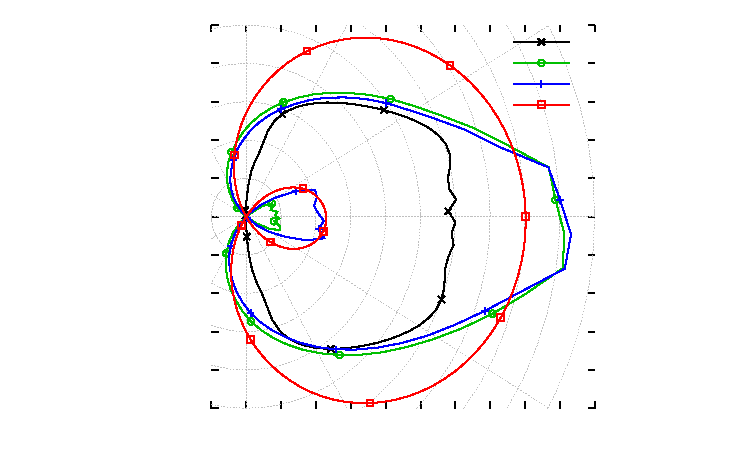
\includegraphics{/Users/seth/_thesis/figures/crashpipe2b/intens-x1-t1/intensity-x1-t1.pdf}}%
    \gplfronttext
  \end{picture}%
\endgroup

  \hspace{-.5in}
  \caption{Scalar flux with a normally incident boundary condition.}
  \label{fig:delta}
\end{figure}
\end{frame}

\begin{frame}
\begin{figure}[tb]
  \centering
  \hspace{-.5in}
  % GNUPLOT: LaTeX picture with Postscript
\begingroup
  \makeatletter
  \providecommand\color[2][]{%
    \GenericError{(gnuplot) \space\space\space\@spaces}{%
      Package color not loaded in conjunction with
      terminal option `colourtext'%
    }{See the gnuplot documentation for explanation.%
    }{Either use 'blacktext' in gnuplot or load the package
      color.sty in LaTeX.}%
    \renewcommand\color[2][]{}%
  }%
  \providecommand\includegraphics[2][]{%
    \GenericError{(gnuplot) \space\space\space\@spaces}{%
      Package graphicx or graphics not loaded%
    }{See the gnuplot documentation for explanation.%
    }{The gnuplot epslatex terminal needs graphicx.sty or graphics.sty.}%
    \renewcommand\includegraphics[2][]{}%
  }%
  \providecommand\rotatebox[2]{#2}%
  \@ifundefined{ifGPcolor}{%
    \newif\ifGPcolor
    \GPcolortrue
  }{}%
  \@ifundefined{ifGPblacktext}{%
    \newif\ifGPblacktext
    \GPblacktexttrue
  }{}%
  % define a \g@addto@macro without @ in the name:
  \let\gplgaddtomacro\g@addto@macro
  % define empty templates for all commands taking text:
  \gdef\gplbacktext{}%
  \gdef\gplfronttext{}%
  \makeatother
  \ifGPblacktext
    % no textcolor at all
    \def\colorrgb#1{}%
    \def\colorgray#1{}%
  \else
    % gray or color?
    \ifGPcolor
      \def\colorrgb#1{\color[rgb]{#1}}%
      \def\colorgray#1{\color[gray]{#1}}%
      \expandafter\def\csname LTw\endcsname{\color{white}}%
      \expandafter\def\csname LTb\endcsname{\color{black}}%
      \expandafter\def\csname LTa\endcsname{\color{black}}%
      \expandafter\def\csname LT0\endcsname{\color[rgb]{1,0,0}}%
      \expandafter\def\csname LT1\endcsname{\color[rgb]{0,1,0}}%
      \expandafter\def\csname LT2\endcsname{\color[rgb]{0,0,1}}%
      \expandafter\def\csname LT3\endcsname{\color[rgb]{1,0,1}}%
      \expandafter\def\csname LT4\endcsname{\color[rgb]{0,1,1}}%
      \expandafter\def\csname LT5\endcsname{\color[rgb]{1,1,0}}%
      \expandafter\def\csname LT6\endcsname{\color[rgb]{0,0,0}}%
      \expandafter\def\csname LT7\endcsname{\color[rgb]{1,0.3,0}}%
      \expandafter\def\csname LT8\endcsname{\color[rgb]{0.5,0.5,0.5}}%
    \else
      % gray
      \def\colorrgb#1{\color{black}}%
      \def\colorgray#1{\color[gray]{#1}}%
      \expandafter\def\csname LTw\endcsname{\color{white}}%
      \expandafter\def\csname LTb\endcsname{\color{black}}%
      \expandafter\def\csname LTa\endcsname{\color{black}}%
      \expandafter\def\csname LT0\endcsname{\color{black}}%
      \expandafter\def\csname LT1\endcsname{\color{black}}%
      \expandafter\def\csname LT2\endcsname{\color{black}}%
      \expandafter\def\csname LT3\endcsname{\color{black}}%
      \expandafter\def\csname LT4\endcsname{\color{black}}%
      \expandafter\def\csname LT5\endcsname{\color{black}}%
      \expandafter\def\csname LT6\endcsname{\color{black}}%
      \expandafter\def\csname LT7\endcsname{\color{black}}%
      \expandafter\def\csname LT8\endcsname{\color{black}}%
    \fi
  \fi
  \setlength{\unitlength}{0.0500bp}%
  \begin{picture}(7200.00,4320.00)%
    \gplgaddtomacro\gplbacktext{%
      \csname LTb\endcsname%
      \put(1910,400){\makebox(0,0)[r]{\strut{} 0.1}}%
      \put(1910,768){\makebox(0,0)[r]{\strut{} 0.08}}%
      \put(1910,1136){\makebox(0,0)[r]{\strut{} 0.06}}%
      \put(1910,1504){\makebox(0,0)[r]{\strut{} 0.04}}%
      \put(1910,1872){\makebox(0,0)[r]{\strut{} 0.02}}%
      \put(1910,2240){\makebox(0,0)[r]{\strut{} 0}}%
      \put(1910,2607){\makebox(0,0)[r]{\strut{} 0.02}}%
      \put(1910,2975){\makebox(0,0)[r]{\strut{} 0.04}}%
      \put(1910,3343){\makebox(0,0)[r]{\strut{} 0.06}}%
      \put(1910,3711){\makebox(0,0)[r]{\strut{} 0.08}}%
      \put(1910,4079){\makebox(0,0)[r]{\strut{} 0.1}}%
      \csname LTb\endcsname%
      \put(2030,200){\makebox(0,0){\strut{} 0.02}}%
      \csname LTb\endcsname%
      \put(2364,200){\makebox(0,0){\strut{} 0}}%
      \csname LTb\endcsname%
      \put(2699,200){\makebox(0,0){\strut{} 0.02}}%
      \csname LTb\endcsname%
      \put(3033,200){\makebox(0,0){\strut{} 0.04}}%
      \csname LTb\endcsname%
      \put(3368,200){\makebox(0,0){\strut{} 0.06}}%
      \csname LTb\endcsname%
      \put(3702,200){\makebox(0,0){\strut{} 0.08}}%
      \csname LTb\endcsname%
      \put(4037,200){\makebox(0,0){\strut{} 0.1}}%
      \csname LTb\endcsname%
      \put(4371,200){\makebox(0,0){\strut{} 0.12}}%
      \csname LTb\endcsname%
      \put(4706,200){\makebox(0,0){\strut{} 0.14}}%
      \csname LTb\endcsname%
      \put(5040,200){\makebox(0,0){\strut{} 0.16}}%
      \csname LTb\endcsname%
      \put(5375,200){\makebox(0,0){\strut{} 0.18}}%
      \csname LTb\endcsname%
      \put(5709,200){\makebox(0,0){\strut{} 0.2}}%
      \csname LTb\endcsname%
      \put(1330,2239){\rotatebox{-270}{\makebox(0,0){\strut{}x1 center $(1.01,3.5)$}}}%
    }%
    \gplgaddtomacro\gplfronttext{%
      \csname LTb\endcsname%
      \put(4806,3916){\makebox(0,0)[r]{\strut{}S$_{128}$}}%
      \csname LTb\endcsname%
      \put(4806,3716){\makebox(0,0)[r]{\strut{}FLAD$_{64}$}}%
      \csname LTb\endcsname%
      \put(4806,3516){\makebox(0,0)[r]{\strut{}AD$_{64}$}}%
      \csname LTb\endcsname%
      \put(4806,3316){\makebox(0,0)[r]{\strut{}FLD}}%
    }%
    \gplbacktext
    \put(0,0){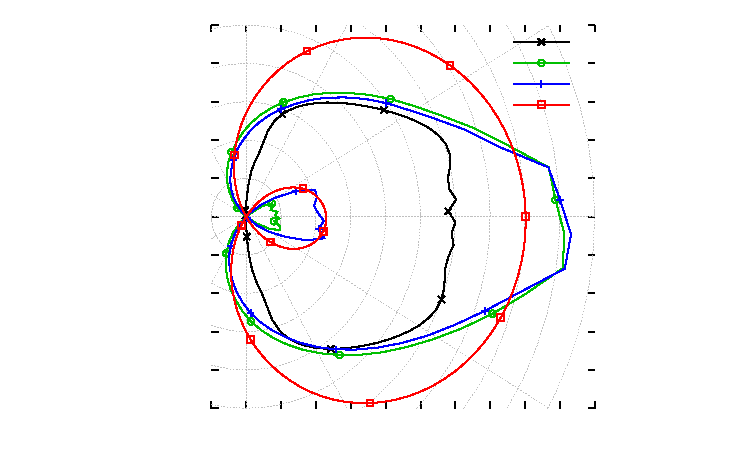
\includegraphics{/Users/seth/_thesis/figures/crashpipe2b/intens-x1-t1/intensity-x1-t1.pdf}}%
    \gplfronttext
  \end{picture}%
\endgroup

  \hspace{-.5in}
  \caption{Relative errors ($\phi/\phi_\text{MC} - 1$) of the three tested
  distributions.}
  \label{fig:relative}
\end{figure}
\end{frame}

%%%%%%%%%%%%%%%%%%%%%%%%%%%%%%%%%%%%%%%%%%%%%%%%%%%%%%%%%%%%%%%%%%%%%%%%%%%%
\section{Conclusions}
\begin{frame}
  \begin{itemize}
    \item We derived Marshak and ``variational'' boundary conditions for
      flatland diffusion
    \item Variational boundaries are more accurate
    \item Generalized form $V(\abs{\vec{\Omega}\vd\vec{n}})$ useful for flatland
      boundary conditions in methods other than diffusion
  \end{itemize}
\end{frame}

%%%%%%%%%%%%%%%%%%%%%%%%%%%%%%%%%%%%%%%%%%%%%%%%%%%%%%%%%%%%%%%%%%%%%%%%%%%%
\begin{frame}
% %\frametitle{Questions?}

{\par\centering\hspace{-.35in}
  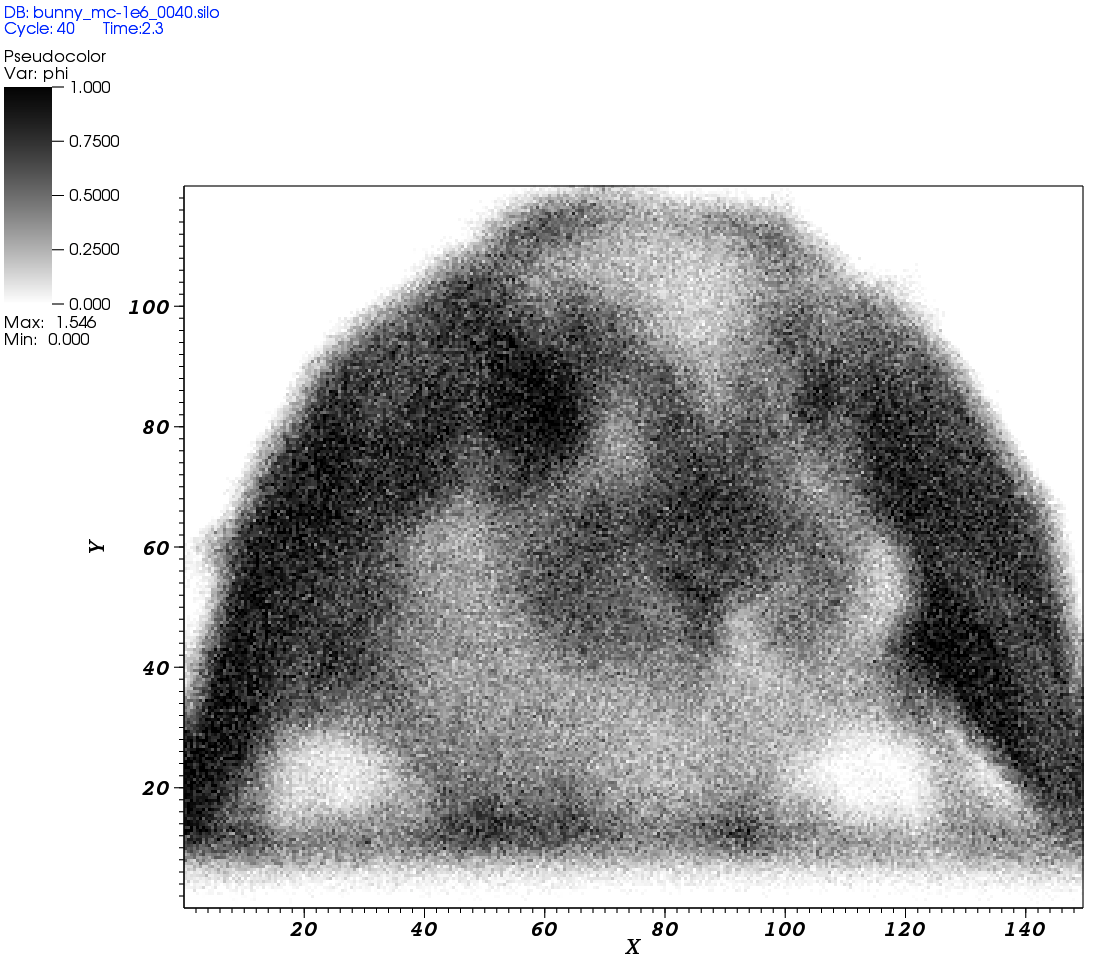
\includegraphics[height=2.75in]{bunny-transport}
  \par}

\vspace{-2.75in}
{\par\centering\Huge Questions?
\par}%
\vspace{2.5in}

{\setlength{\baselineskip}{-\baselineskip} \tiny  \raggedright
This material is based upon work supported under a National Science Foundation
Graduate Research Fellowship and a Department of Energy Nuclear Energy
University Programs Graduate Fellowship. Any opinions, findings, conclusions or
recommendations expressed in this publication are those of the author and do
not necessarily reflect the views of the National Science Foundation or the
Department of Energy Office of Nuclear Energy.\par}
\end{frame}

%%%%%%%%%%%%%%%%%%%%%%%%%%%%%%%%%%%%%%%%
\appendix
\begin{frame}
  \frametitle{References}
\bibliographystyle{ans}
\bibliography{../../SRJall}
\end{frame}
%%%%%%%%%%%%%%%%%%%%%%%%%%%%%%%%%%%%%%%%%%%%%%%%%%%%%%%%%%%%%%%%%%%%%%%%%%%
\end{document}

